\documentclass{article}
\input{../../preamble.tex}
\usepackage[letterpaper, portrait, margin=1in]{geometry}

\graphicspath{./figures}

\pagestyle{fancy}
\fancyhf{}
\lhead{Sidharth Baskaran}
\chead{Project Euler 50}
\rhead{01/10/2022}

\lstset{
	basicstyle=\ttfamily\scriptsize,
	frame=single,
	breaklines=true,
	mathescape
}

\begin{document}
    
\section{Problem Statement}

The prime 41, can be written as the sum of six consecutive primes: $41 = 2 + 3 + 5 + 7 + 11 + 13$
This is the longest sum of consecutive primes that adds to a prime below one-hundred. The longest sum of consecutive primes below one-thousand that adds to a prime, contains 21 terms, and is equal to 953. Which prime, below one-million, can be written as the sum of the most consecutive primes?

\section{Code}

\lstinputlisting[language=Python]{../code/50.py}

\section{Explanation}

The algorithm generates a list of primes below $n$ (\num{1e6} in this case) starting with 2 using the Sieve of Erastothenes, as outlined in the method \verb|get_prime_list|.
A boolean array of length $\num{1e6}+1$ is initially defined with all true values. The sieve then begins by iterating from $i=2$ to $i=\sqrt{n}$ in the outer loop, and the inner loop marks every $i$th array location after $i^2$ false, as defined by the algorithm.
Finally, we select all integers corresponding to remaining true values in the array; these constitute a list of prime numbers.

Before entering the \verb|solve| method, we take a quick look at \verb|is_prime|, a method which
iterates through all numbers less than $\sqrt{n}$ (excluding 1), checking for divisibility. We only have to check from $\sqrt{n}$ and below because at least one factor of a nonprime number is below its square root.

Since the problem asks for the longest consecutive list, we observe the given example hint of $n=1000$.
If we naively start from the beginning of our prime number list, summing until $n$ is exceeded, we do not get the expected result of 953.
Clearly, this simple approach will not work. We need to find \textit{the longest consecutive list} of primes that sum to a prime number, which is not necessarily
the list beginning with 2, as in the simple example of 41, the sum from a list of 6 consecutive primes below 100.

\begin{figure}[H]
	\centering
	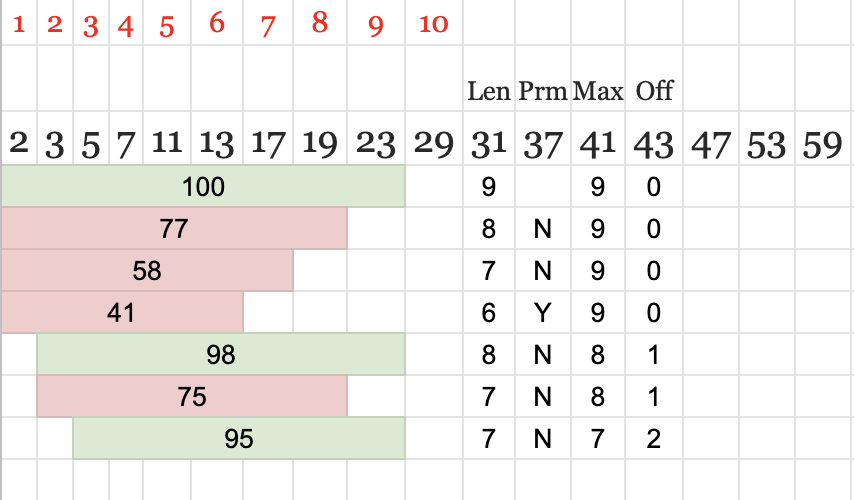
\includegraphics[scale=0.5]{../figures/spreadsheet.png}
	\caption{Visual of main algorithm}\label{ss}
\end{figure}

Figure \ref{ss} visualizes an example with $n=100$, where we want to obtain the . The \verb|solve| method begins
by storing the prime number list. Initially, we obtain the largest possible ``naive'' list
by iterating from 2 to some $x$ in the list of prime numbers $P$ where $\sum_{i=0}^xP[i] \leq 100$.
In the above example, this is the list $2,\ldots,23$ of length 9 which sums to $100$. We store this as our \textit{maximum possible sublist length}.

Then, we iterate through the different possible sublists of length $< 9$. Our outer loop increments a 
left offset that we can see easily in the above example. This helps us permutes through all possible starting points for sublists. It also checks to make sure the next sublist length will not fall below a threshold value defined by our current maximum sublist length (initialized to 0), since there is no point looking for smaller sublists than the maximum we will find.
On each outer loop iteration, we enter an inner loop. We start with a sublist, denoted in green, check for primality,
then successively decrease the sublist size using a ``right offset'' until we reach the maximum sublist length previously determined (initialized as 0). If the sublist sums to a prime number, we make sure it doesn't exceed a prior maximum and record it as the ``best sum'' and new maximum length.

\begin{figure}[H]
\centering
\begin{BVerbatim*}
997651
296.665ms
\end{BVerbatim*}
\caption{Output}
\end{figure}

\end{document}